% If you want to compile this section only, make sure to include relevant document headers and the \being \end document commands.
% You can make this a bit easier if you use the subfile package

A pilot study has been conducted to understand how external (locational) features and internal (property) features influence housing prices based on a machine learning algorithm. In the pilot study, features related to property location/environment include park proximity, hospital proximity, and geotag (latitude and longitude). Features related to the property itself include bedroom size, bathroom size, and built year. The correlation heat map (Figure 2) shows that both internal and external features appear in the top positively and negatively correlated features to housing prices. Two major findings from the machine learning tasks are:

\begin{itemize}
    \item In tree-based models and regression models, both internal and locational features contribute to the housing price prediction.
    \item In linear regression models (Poly 2), locational features are of higher importance, especially latitude, which reflects the North-South segregation in Chicago.
\end{itemize}

\begin{figure}[h]
    \centering
    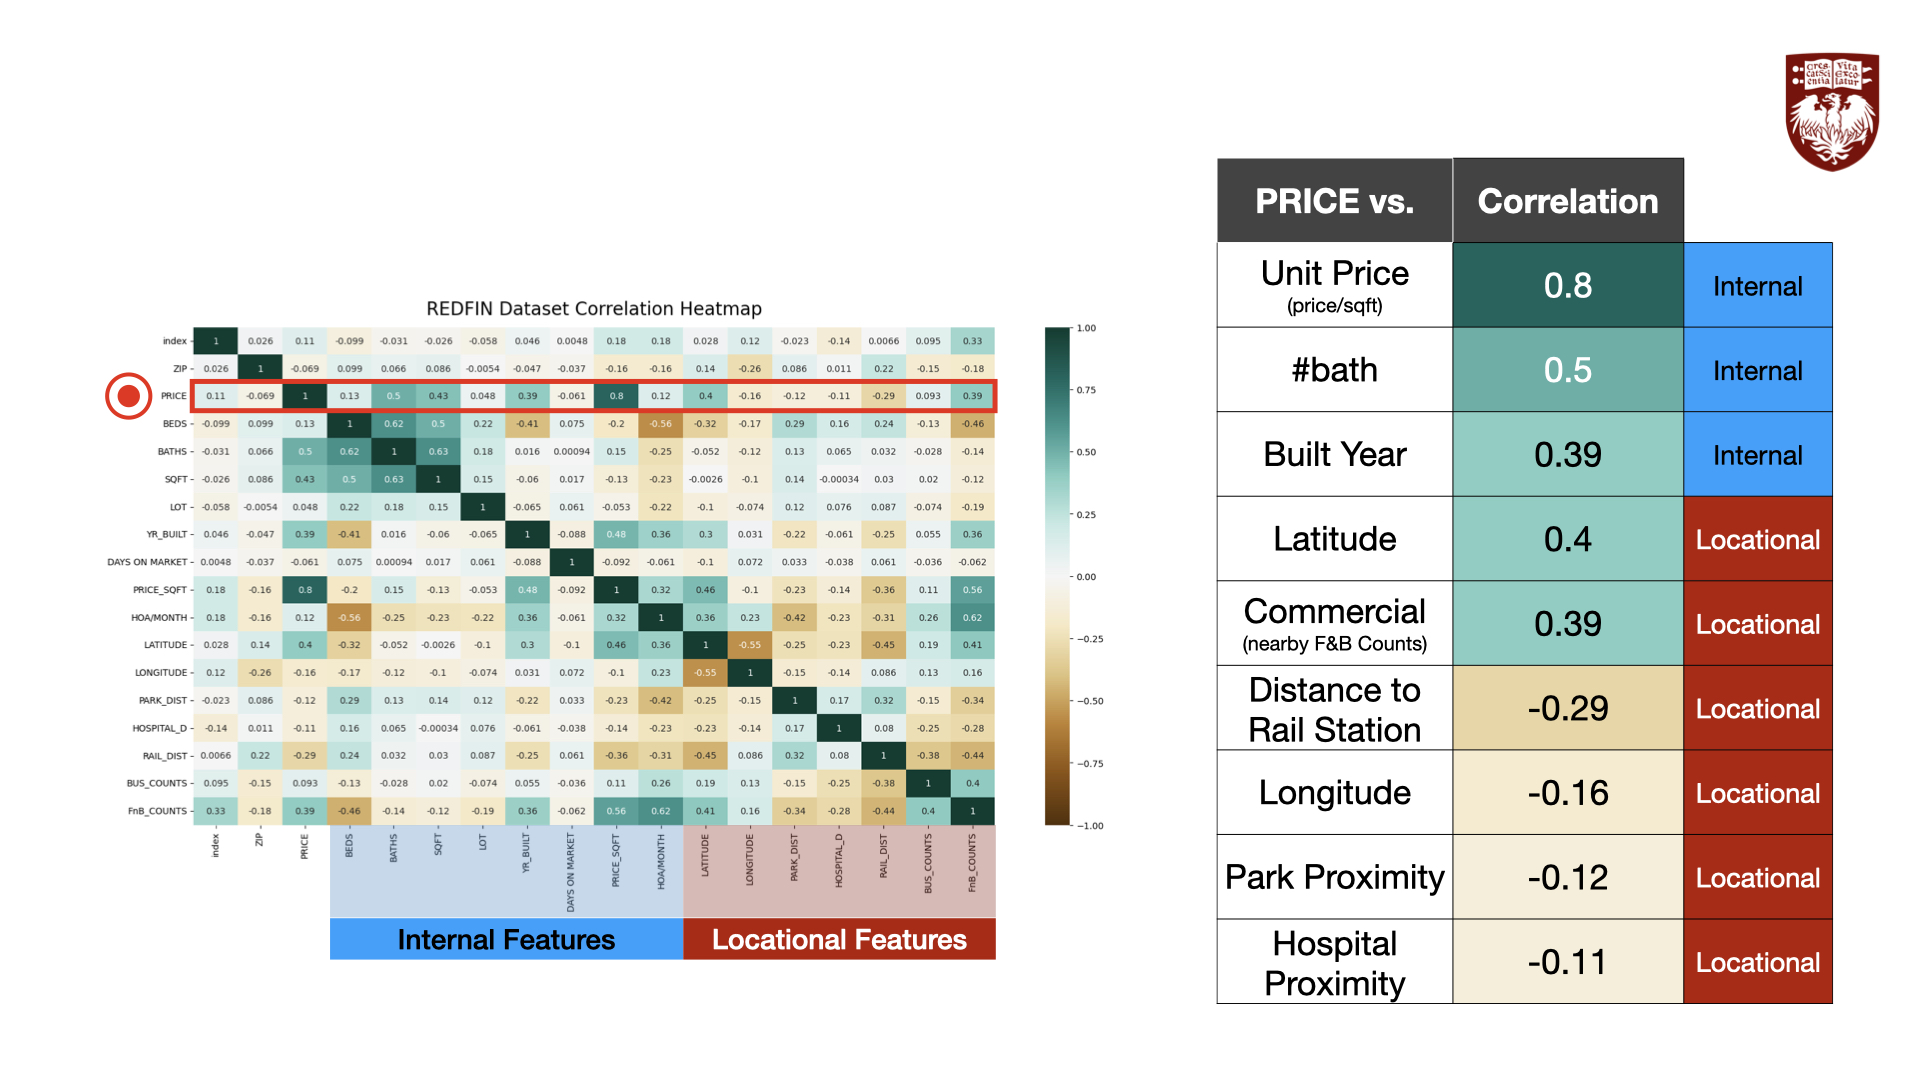
\includegraphics[width=1\textwidth]{Visual/final_heatmap.jpeg}
    \caption{Coorelation Heat Map}
\end{figure}

According to the error analysis, my model is more likely to underestimate high-price properties than to overestimate low-price properties (Figure 3).

\begin{figure}[h]
    \centering
    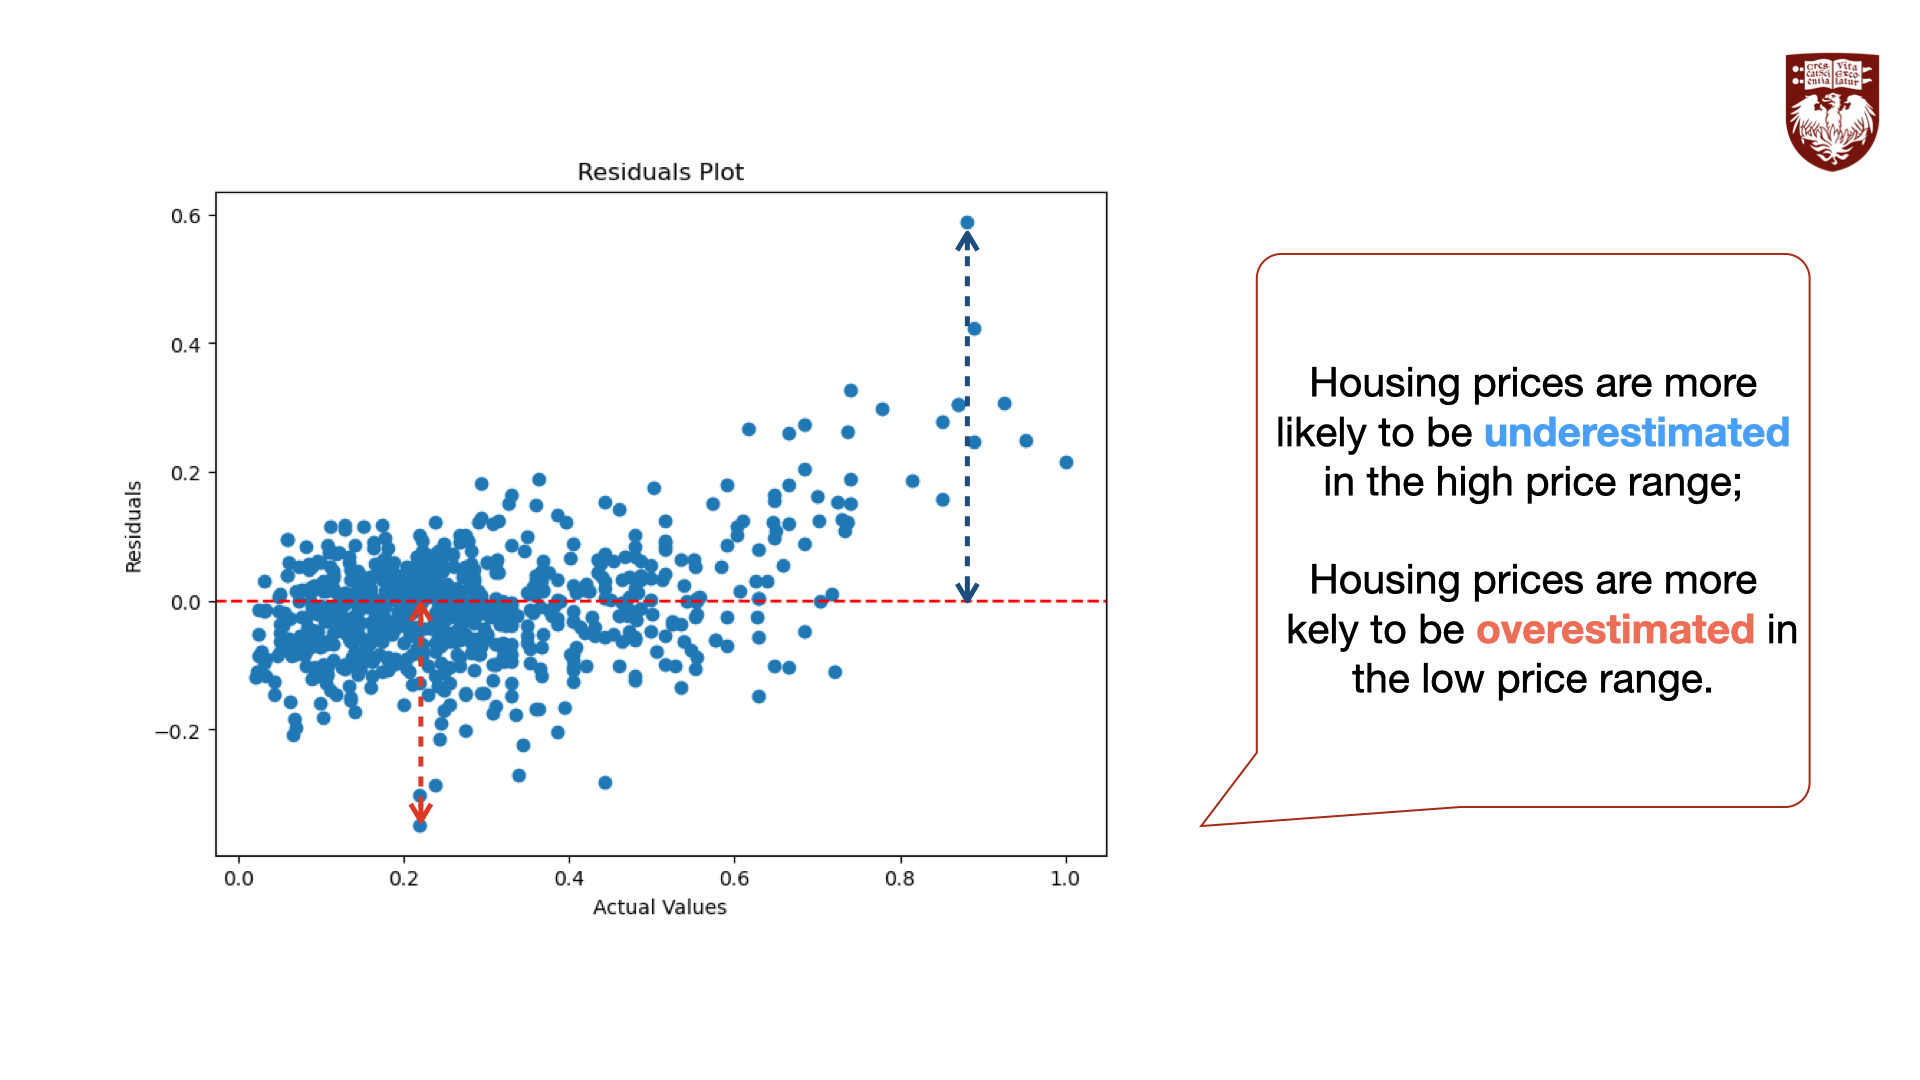
\includegraphics[width=1\textwidth]{Visual/final_error.jpeg}
    \caption{Error Analysis}
\end{figure}

However, the proximity to the park shows a negative correlation to housing prices, which does not align with previous studies that utilized the hedonic regression model in my literature review. There are three major potential problems in analysis:

\begin{enumerate}
    \item The feature proximity to the park is based on the distance from each listing to the nearest park space retrieved from the governmental database. The database does not include minor green space and private green space. The feature does not reflect the natural green space environment near the listings.
    \item According to the map of the error analysis (Figure 4), most underestimation cases appear in the city center area. This might be related to the functionality of UGS in the city center. Downtown UGS is usually associated with a higher homeless population and potential security problems. People living downtown might have a different preference from people living in the city fringe.
    \item Chicago is a city with significant North-South segregation, so the latitude feature shows an extremely high coefficient, which might influence the significance of all the other features in the regression model.
\end{enumerate}

\begin{figure}[h]
    \centering
    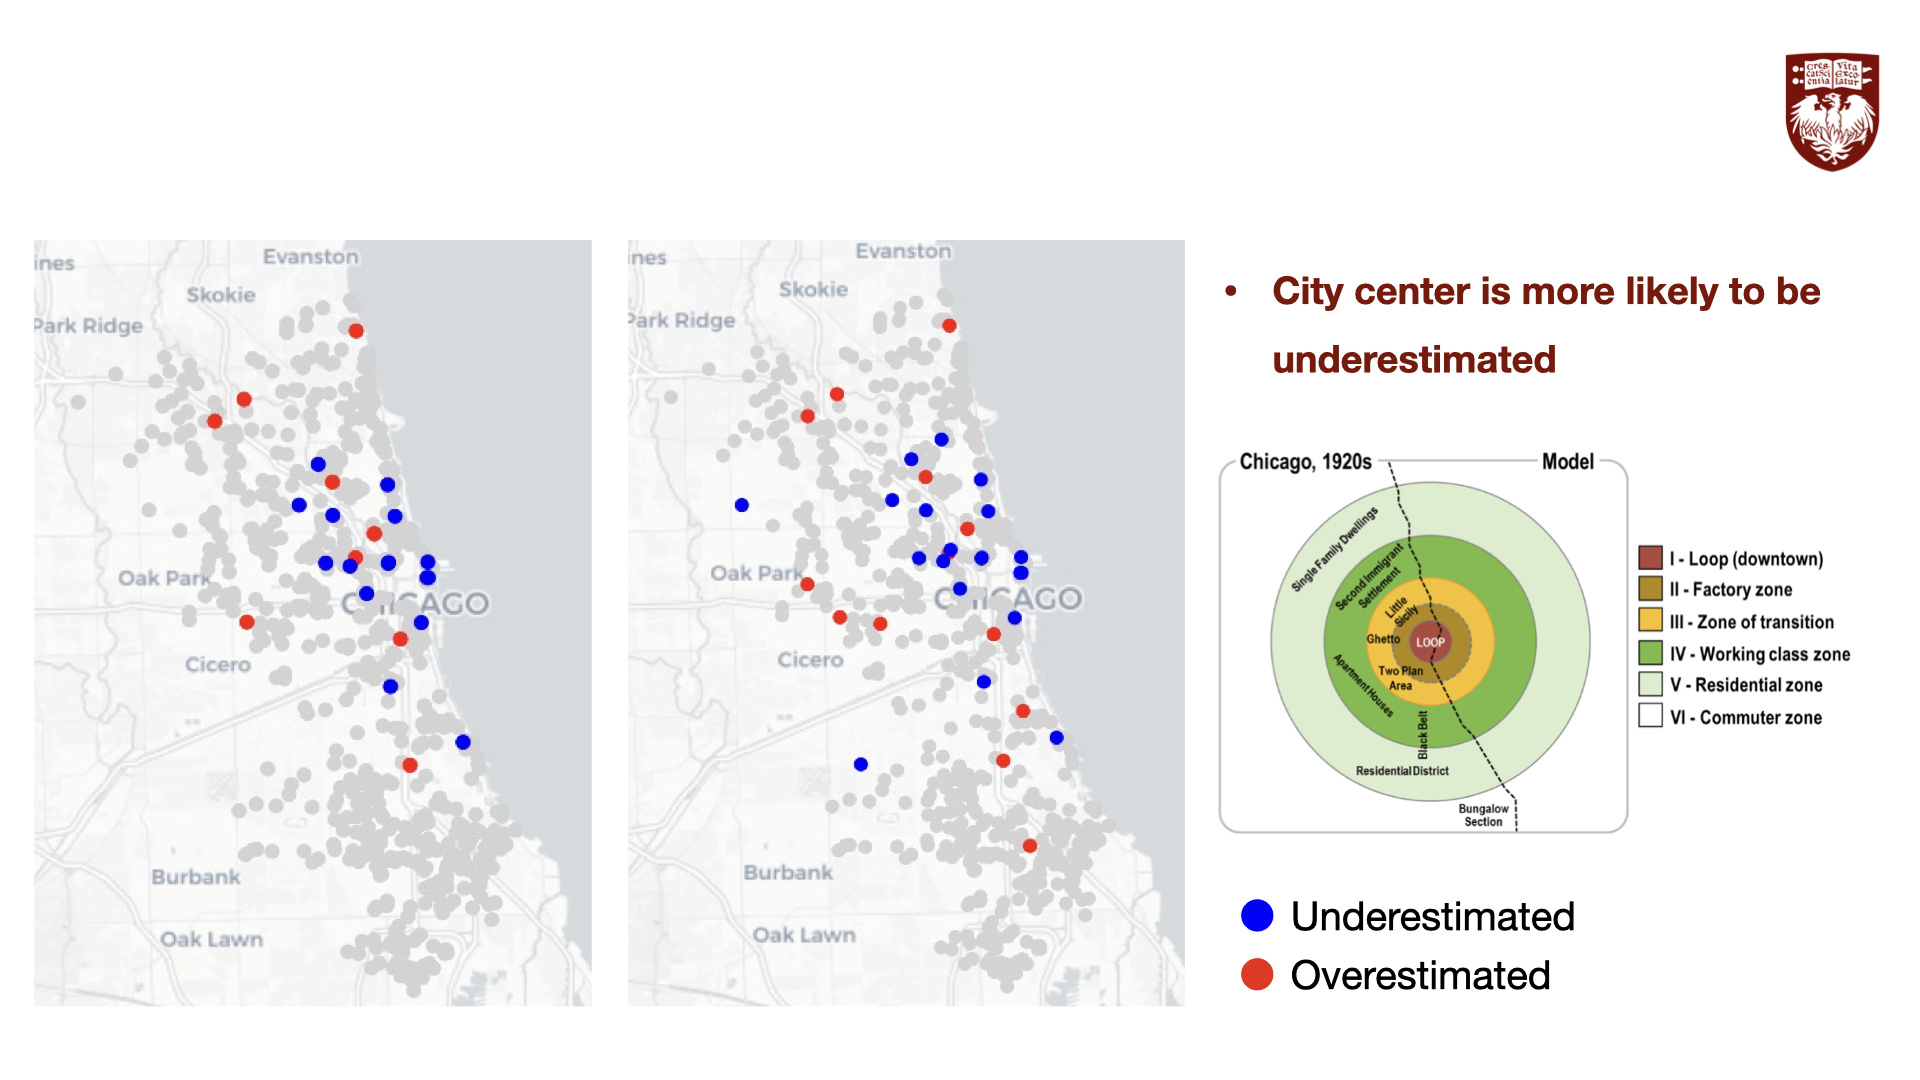
\includegraphics[width=1\textwidth]{Visual/final_map.jpeg}
    \caption{Error Analysis Map}
\end{figure}

To address these problems, I will adopt the new data processing methodology using the NDVI calculation based on satellite imagery in my next step of research. The NDVI calculation will provide an objective analysis of how much green space the residents can interact with daily. For people’s different living preferences between the city center and city fringe, I plan to run machine learning models separately on different neighborhoods to understand the disparities within the city. Lastly, I will remove some of the significant features in the previous machine learning task to better examine the correlation between housing price and UGS distribution.